\documentclass{article}
\usepackage{graphicx}
\usepackage{dot2texi}
\makeatletter
\@ifundefined{verbatim@out}{\newwrite\verbatim@out}{}
\makeatother
\usepackage{tikz}
\usepackage{hyperref}
\usetikzlibrary{shapes,arrows}
% \usepackage[pdf]{graphviz}
%\usepackage{feynmp}
\usepackage{subfigure}
\usepackage{dsfont}
\graphicspath{{figs/}}

\title{Spark Notes}

\author{Peter Thompson}

\begin{document}


\section{Links}
\subsection{joining}
    \begin{itemize}
        \item \url{https://databricks.com/session/optimizing-apache-spark-sql-joins} 30 minute video, good overview
        \item \url{https://sujithjay.com/spark-sql/2018/02/17/Broadcast-Hash-Joins-in-Apache-Spark/} part one of a series
    \end{itemize}
\subsection{catalyst}
 \begin{itemize}
        \item \url{https://databricks.com/session/deep-dive-into-catalyst-apache-spark-2-0s-optimizer} deep dive into catalyst
        \item \url{https://databricks.com/blog/2015/04/13/deep-dive-into-spark-sqls-catalyst-optimizer.html} databricks blog post
        \item \url{http://people.csail.mit.edu/matei/papers/2015/sigmod_spark_sql.pdf}
    \end{itemize}

\section{Questions}
\begin{itemize}
    \item {\bf Tasks/cores/executors}
    \begin{itemize}
        \item in databricks, can we specify only 2 (for instance) executors for a node with 8 cpus?
        \item if so, are these executors/jvms aware that the node has more cpus available? Are they accessible
        Use case - want to run some non-spark multithreaded code, e.g. distribute 1 xgboost job to each node, with each job using c cores
        \item Ali said that he turned off autoscaling and had one executor per node. (8 cores per node)
    \end{itemize}
    \item {\bf joining} 
        We have (say) a small list of collector ids, and want to left join with 5-6 large tables (millions of collector ids, thousands of columns)
        What is the best (optimal) way to do this? More shuffle partitions are better? more data partitions?  
    \item {\bf joining also} - Build/stream? what are these? is this for hashing?

\end{itemize}

\section{Joining}
    

    \subsection{Shuffle Hash join}
    Pretty (most?) common type of join. Data from table 1 and table 2 are partitioned by key. Matching partitions are sent to the same executor, then the output is merged.
    This works best when
    \begin{itemize}
        \item data is evenly distributed by key
        \item good number of keys (unique values - monthid would be a bad key (12 unique values))
    \end{itemize}
    When these conditions can't be satisfied, then broadcast hash join might be suitable
    NOTE spark config option,\verb|spark.sql.join.preferSortMergeJoin|, (set true by default), essentially means that Sort Merge join is always chosen over shuffle hash join


    Diagnosing problems
    \begin{itemize}
        \item Tasks that take a long time - could be uneven sharding (keys not distributed evenly).
        \item Speculative tasks - if something takes a long time on one exdecutor, spark might send think theres a problem there and send the task to another to see if ti works there. If one particular task spawns speculative tasks, this can also be a sign that there is a sharding problem.
        \item Shuffle read/write memory - take a look to see if there is one task sending/receiving a lot of data (more than average)
        \item ls across the output files - see if one data partition is much larger than others
    \end{itemize}

    \subsection{broadcast hash join}
    Small table sent to every executor, each partition is joined with the entire table, then output is returned. Bestest performance. Spark will automatically broadcast tables that are smaller than \verb|spark.sql.autoBroadcastJoinThreshold|, which is 10 MB by default. Giving hints can override this behaviour, but if the broadcasted table is too big you may OOM your cluster.
    For right outer join, Spark can only broadcast the left side. For left outer, left semi, left anti and the internal join type ExistenceJoin, Spark can only broadcast the right side. I have had cases where I want to join a small list of collectors, tableA, (one column of collector keys) to a bigger table (millions of rows, thousands of columns). Normally I would do \verb|c = tableA.join(tableB,['COLLECTOR_KEY'],how='left')|. To use broadcasting, the join has to be righted: \verb|c = tableB.join(broadcast(tableA),['COLLECTOR_KEY'],how='right')|. 

    \verb|df.explain()| on the output will tell whether a shuffle hash or broadcast hash join is being made
    (spark can sometimes have a hard time figuring out when to use a broadcast join with stuff in hive. giving a hint might be handy).

\subsection{Cartesian join (cross join)}
\begin{itemize}
    \item create an rdd of uid by uid pairs
    \item broadcast that
    \item call a udf that retrieves data from the big tables given the uid,uid pairs
\end{itemize}

\subsection{one to many join (one sided cartesian)}
- number of rows can explode
not a big deal with parquet - duplicate data encodes well (for output files)

\subsection{theta join}
join tableA with TableB on (keyA < keyB +10)
  - Spark will treat this as a cartesian join
  - Much better to bucket A and B, and create an intial paritioning based on bucket equality

\section{rough}

\section{parallelism }
Spark runs on clusters. A cluster has one driver, and a bunch of nodes. Each node has one or more executors, and each executor has one or more slots. A slot is a ``virtual'' cpu core, when spark is running things, it will distribute the tasks to executors, and each executor will simultaneously run one task for each slot. Can think of these as cpu cores, but the number of slots is configurable (could have 6 physical cores and specify only 4 slots) (spark calls slots ``cores'', but databricks training referred to them as slots to avoid ambiguity). 

Each executor is a process that runs on a worker node. Each slot is a seperate JVM managed by the executor process with some amount of resources allocated. 

Data is parallelised also. Whenever a csv or parquet file is read in, the data is split into partitions and distributed amongst slots. If the input file was partitioned, then spark will use these partitions and distribute them amongst the slots. If the data is not partitioned (i.e. a single file, or multiple independant files), then spark will divide it into partitions and distribute them automatically (it will try to be smart about this).


\section{Transformations and Actions}
There are two types of operations in spark, transformations and actions. Transformations are lazy, which means when they are invoked, nothing actually happens. Spark figures out what you want to do and makes a note of it. Actions are eager, when an action is invoked, spark realizes that it needs to touch the data, so it backtracks through the lineage of the dataframe (back to the input), computes all the transformations and returns a result. Theres a bunch of optimisation (see catalyst below) steps that happen first, but these aren't executed untill you invoke the action.

\subsection{Narrow and Wide transformations}
Data in spark is partitioned. That is, each executor slot holds some pieces of the data. Transformations can be either narrow or wide. A narrow transformation is one in which there is a one to one mapping between input and output partitions of data. That is, the transformation can be applied to one input partition to create one partition of the output dataset. 


\begin{figure}[hbpt]
    \subfigure[narrow transformation]{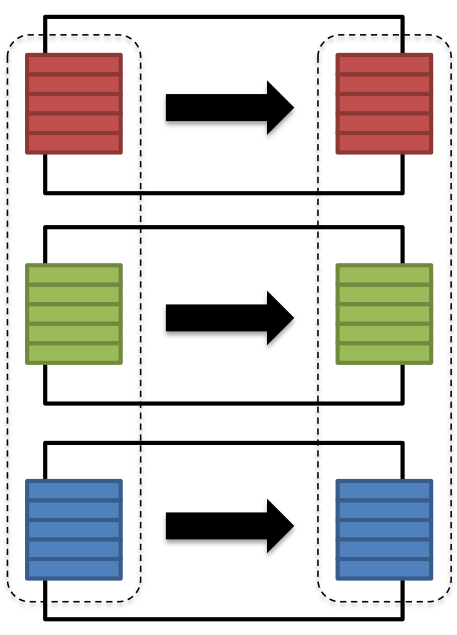
\includegraphics[width=0.45\textwidth]{transformations-narrow.png}}
    \subfigure[wide transformation]{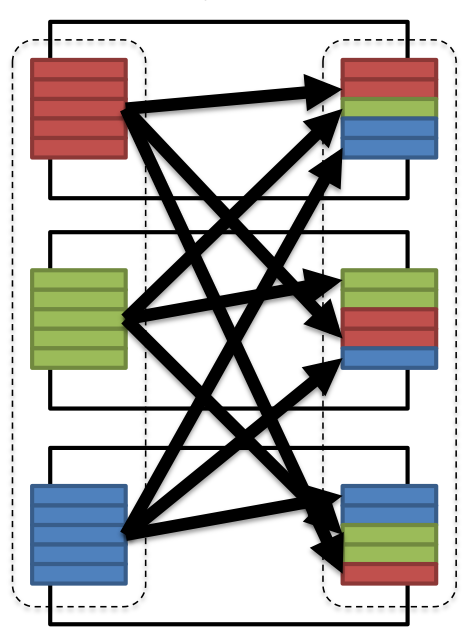
\includegraphics[width=0.45\textwidth]{transformations-wide.png}}
    \caption{narrow (a) and wide (b) transformations. A narrow transformation has a one to one mapping from input to output data partitions. Output partitions from a wide transformation depend on multiple input partitions (shuffle)}
\end{figure}

Narrow transformations are great. Spark (catalyst) will pipeline things, optimising sequences of narrow transformations as much as possible. Narrow transformations are extremely parallelisable, as they are performed independantly across each partition. If there is at least one data partition for each available slot, then these will scale very well.

In order to carry out a wide transformation, data needs to be shared amongst partitions. This involves a shuffle, which is an expensive operation. For example, consider
\begin{verbatim}
df.groupBy('COLLECTOR_KEY').agg(F.sum(F.col('AMRM_EARNED'))
\end{verbatim}
You can get an idea of the execution plan by using the df.explain() function. The aggregation above requires spark to first create partial sums (by collector key) over eah partition, then distribute the data so that all of the partial sums for each collector key end up in the same shuffle partition. Each shuffle partition then sums by collector key again to get the final totals. 

Shuffling involves two exhange operations. First, data on a partition is broken up into different pieces, one for each of the shuffle partitions that will be used. Each of these pieces is written to disk. The second part involves executors (slots) pulling the data that they need from other slots. These are then merged into a single partition, and data processing continues. 

When shuffling, spark needs to figure out where a given piece of data will go (partial sum by collector key in the above example). This is a mapping from a key to a shuffle partition, which is done by a hash function. Spark will use rangepartitioning (hashpartitioning) to figure out how to map data to shuffle partitions {\bf if} the number of shuffle partitions is less than 200. In these cases hashpartitioning is optimal and works best. If there are more than 200 shuffle partitions then sortmerge partitioning is used. Ideally you want less than 200 shuffle partitions.


% exchange rangepartitioning  (hashpartitioning)- the efficient one that can be done if shuffle partitions is less than 200 




\subsection{actions}
For Dataframes, there are three types of actions
\begin{itemize}
\item actions to view data in the console (.show(), display in databricks)
\item actions to collect results at driver (collect())
\item actions to write data (write)
\end{itemize}

With dataframes, any function that acts on a dataframe and returns a dataframe is a transformation (filter, withColumn, select, etc). Any function that returns something other than a dataframe is an action (collect, write, show, count). Transformations tell spark how to change data, actions tell spark what to do with the data. 

% Transformations
% narrow transformations are where each input partition contributes to one output partition.
% Spark pipelines stuff - in narrow transformations, things like filters are all performed in memory.
% Wide transformations are those where a SHUFFLE is required, an output partition requires data from multiple input partitions.
% Shuffles transfer data across the network, and results are written to disk.

% lazy evaluation
% spark doesn't do anything untill you need a result. Predicate pushdown - if you filter at different stages, these get pushed down as far as possible, so spark only deals with the minimum amount of data required. This allows for lots of optimisation

% Actions
% There are three types of actions
% - actions to view datsa in the console (.show(), display in databricks)
% - actions to collect results at driver (collect())
% - actions to write data (write)

% Explain can be called on any dataframe. It will show the physical plan for processing the data to carry out all the transformations. The top of the plan is the end result, the bottom are the inputs. The logical plan is the set of transformations specified, the physical plan is what spark will do to get the result, 


\subsection{lazy Evaluation}
\subsection{catalyst}
\begin{figure}[hbpt]
    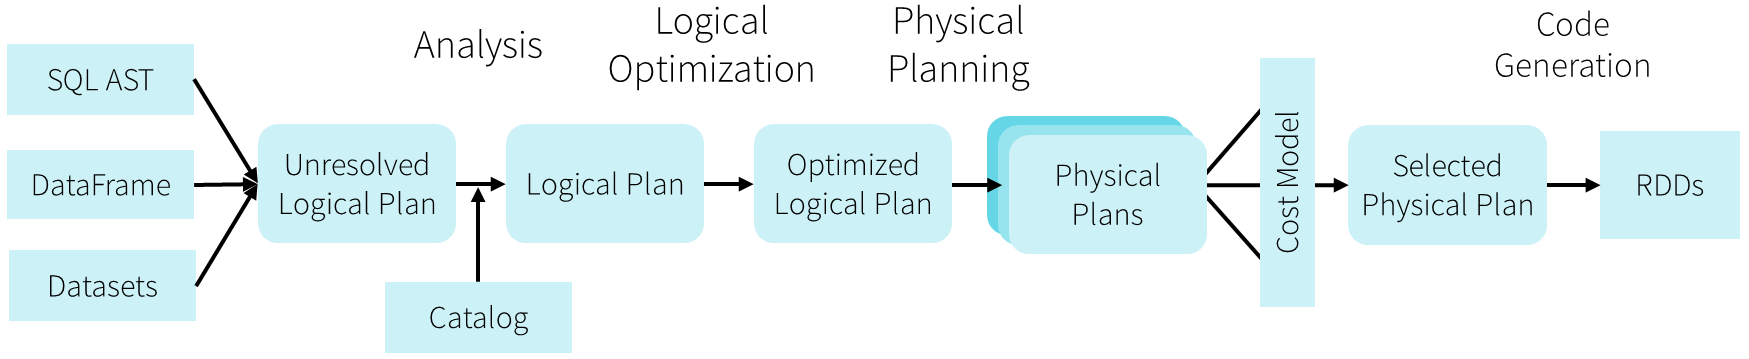
\includegraphics[width=0.9\textwidth]{catalyst-diagram.png}
    \caption{schematic illustrating the steps taken by catalyst in order to determine execution plan}
    \label{fig_catalyst_diagram}
\end{figure}

\subsection{DAG - job/stage/task}
Spark jobs are initiated when actions are invoked. Each job is broken down into one or more stages, and each stage is comprised of multiple tasks.
A task is a piece of work - operations that run within a single partition of data. A stage is a set of tasks that can be run without exchanging any data (i.e. narrow transformations). When data needs to be shuffled, then the stage will end in an exchange operation, where each partition divides the data it has processed into shuffle partitions and writes these to disk. The first step of the next stage involves each shuffle partition pulling the data that it needs from other slots, and merging these together.

The Directed Acyclic Graph illustrates the flow of data. Stages are seperated horizontally in the DAG, with a red box around them. Wavy arrows going from one box to another indicate shuffles.

\begin{figure}[hbpt]
    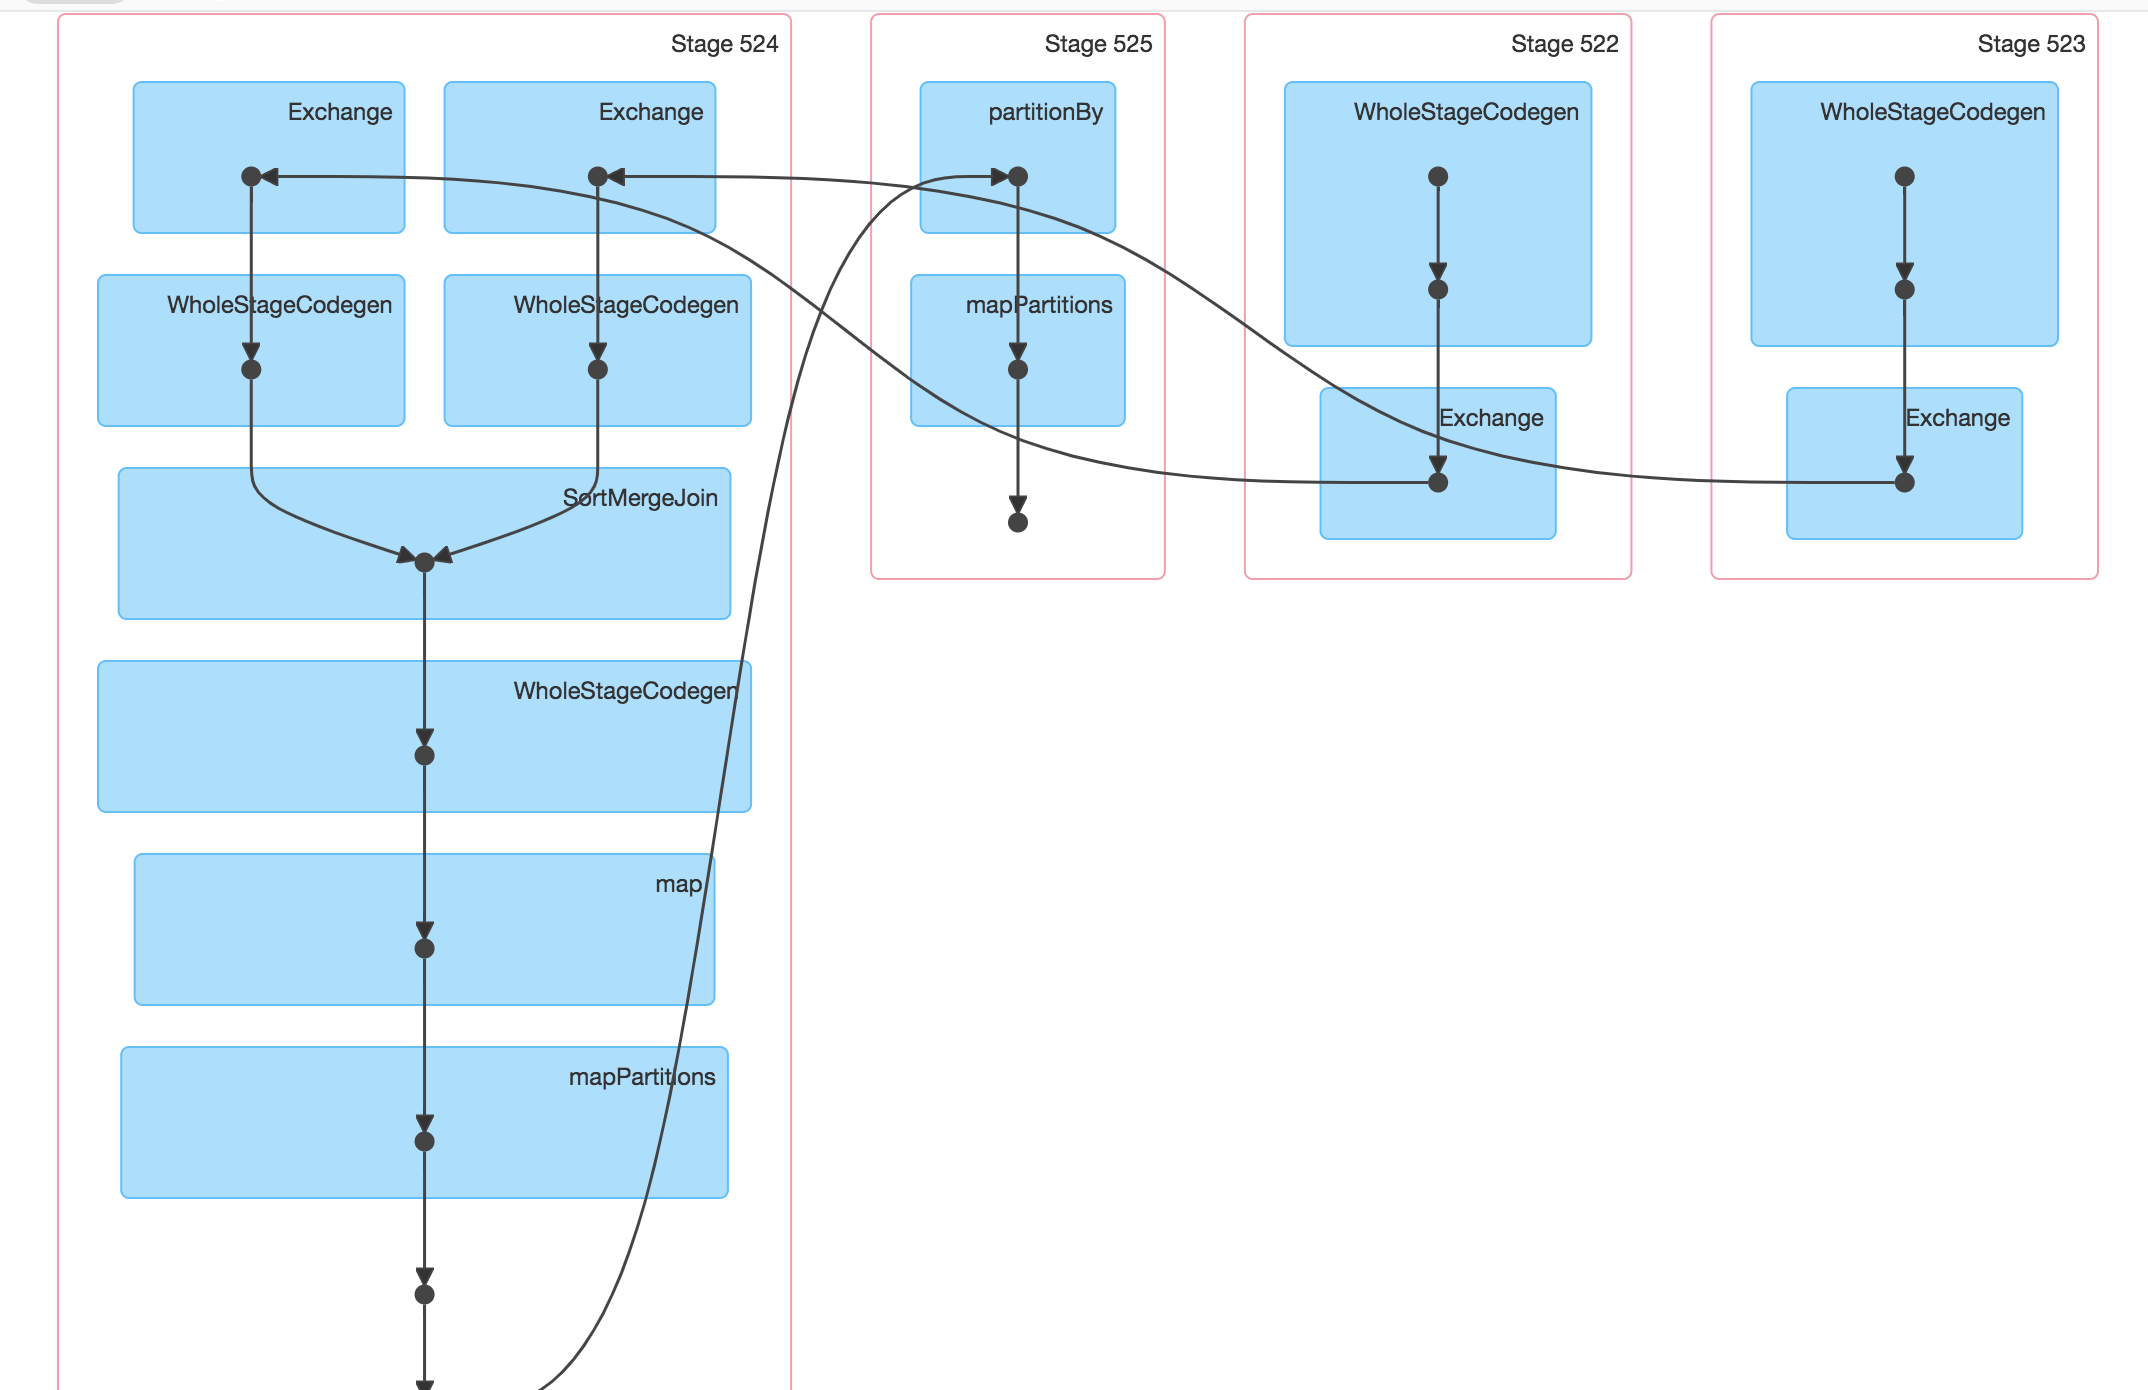
\includegraphics[width=0.6\textwidth]{DAG.png}
    \caption{Directed Acyclic Graph (DAG) from a spark job. Stages are bounded by red boxes, wavy arrows between red boxes indicate shuffles (these arrows begin and end on exchange operations). }
    \label{fig_dag_example}
\end{figure}

% #### RoughRough


% ###################################
% berkely amp lab

% started by Matei Zaharia. Was working on netflix prize using mapreduce, tried to make it better and invented spark, tied for netflix prize, but ended up second.
% certification

% catalyst optimiser - spark dataframes can be 5-20X faster than regular RDDs
% yet another resource negotiater

% Performance - dataframe performance is really good, and there is no difference between python, scala, R or SQL. When working with RDDs, Scala performs better than Python (about 2x)
% Catalyst - binds python (or R or SQL) dataframe functionality to scala based operations. Fast

% architecture - driver -> executor -> slot. Typically worker nodes have one excutor, and that has one slot (process thread) per cpu available


% Jobs are made of stages
% each stage is the set of operations that can be run in parallel without dependencies (shuffling)

% databricks - REPL shell
% displayHTML - can pretty display things


% anytime you create a spark session (dataframe interface stuff), a spark context named sc is created automagically

% documentation for spark - python and scala are maintained by different people, check scala docs if python ones seem to be lacking

% jobs created when spark needs to touch data
% When you spark.read, this is not an action
% a job is created, and run eagerly, on spark.read. This is to get an idea of the schema

% nullable things in schema aren't used by spark, but are to maintain compatibility with other databases (parquet?)

% parquet
% google dremel project - released white paper, desxcribes file format
% parquet derived from this
% preserves dataframe info - both metadata and row/column data

% read.parquet executes (eagerly) one very small spark job to read metadata. read.csv reads entire file (all data)
% can specify the schema even for parquet files, this avoids the (small) job to read metadata

% # Dataframes
% anything that returns not a dataframe is an action. triggers evaluation

% dataset - rdd of type specific stuff. Stringly typed. Collection of classes.
% Not available in python, only have dataframes. Dataframes are datasets of row objects. One row may have different columns to another. 

% Caching - when an action is called, spark figures out the lineage (physical plan? logical plan?) and builds the dag. When it hits some data that's been cached then it uses that and does not go back further.


% #Transformations and actions
% Narrow transformatoins are those that do not require a shuffle. The transformation can happen within each partition
% Wide transformations require data from other partitions. These require a shuffle
% A stage is a set of jobs that happen within partitions. A set of narrow transformations. 
% green dots in the dag are cache points

% Catalyst Optimiser
% sequence of api calls and action -> unresolved logical plan -> check catalog (from hive, make sure all columns exist) -> resolved logical plan -> optimised logical plan (first pass, move filters down) -> series of physical plans (lots of paths to get the same result) -> check cost of each plan -> choose best -> do stuff, result (runs on rdds)
% udfs can screw up optimisation.
% catalyst assumes udfs run in jvm (judf is in java or scala )
% python udfs are particulary difficult. Data may need to be taken out of the jvm, run through a python interpreter, put back into jvm and back into dag.
% python udfs are bad.

% https://spark-summit.org/2016/events/deep-dive-into-catalyst-apache-spark-20s-optimizer
% https://www.youtube.com/watch?v=6bCpISym_0w
% https://databricks.com/blog/2015/04/13/deep-dive-into-spark-sqls-catalyst-optimizer.html
% http://people.csail.mit.edu/matei/papers/2015/sigmod_spark_sql.pdf


% catalyst2
% explain()
% += indentations denote different stages
% filter drops nulls by default (filter on col != val) will drop nulls
% Predicate push down - when reading parquet, jdbc, etc (NOT CSV), filters get pushed down right to the very begining, as we read data from the source (only read what we need). Cache can screw this up. If we cache the entire table, and then



% Wide and Narrow
% Wide transformations shuffle data. If we are using 4 shuffle partitions, then for each datapartition we hash data into 4 partitions, and write out a file for each partition. Then we send each file to the corresponding executor.  GetPartition is the function that figures out which shuffle partition a record goes into


% Cache can screw things up. If data is cached in the middle of a pipeline, then spark can't push predicates(filters) down past there. In some cases, removing the cache means the filter can move right to the beginning, which speeds up a bunch of stuff

% spark will combine as many narrow operations as it can into a single task

% Caching before a shuffle is pointless. Spark will track back from the action to the shuffle, and get to the files on disk, those sent to the node on the second part of the shuffle. It will never go back through the shuffle to reach the cache. The transformations and actions notebook has some of this

% *** Jobs/Actions - one job per RDD ACTION. Catalyst will take the dataframe code (API), run it throguh catalyst and get an optimised logical plan (which is formed in terms of transformations and actions on the underlying RDD). There is one spark job per RDD action in the optimised plan. So a sequence of dataframe transformations may result in a single (dataframe) action, which is optimised to multiple RDD actions, resulting in multiple jobs

% ** Caching
% articulation - shuffle
% Persistance/caching - disk only/disk only 2 - 2 copies on disk
% memory and disk is actually memory or disk, if there is no room in memory then it is spilled to disk
% memory and ser - serialisation - can set up spark to use kyro or java serialisation (rather than default tungsten)
% dataframes are memory and disk by default. this is good for resilience, almost guaranteed to be able to sucessfully cache

% spark spark.catalog.cachetable vs df.persist?
% tuning 11 - the overhead of caching - take a look at this
% cacheas - in tuning 13
% cache can break predicate push down, if you readparquet, cache, then filter, it may be slower than just read.parquet.select.filter, because parquets are awesome and spark will just read what it needs. when you insert a cache, spark wants to remember the entire dataframe, so it needs to read the entire table from parquet (then cache, then filter)

% # Spark settings
% spark context
% theConfig = sc._conf.getAll()
% print('\n'.join(['{k}: {v}'.format(k=x[0],v=x[1]) for x in theConfig if 'emory' in x[0]]))
% spark.config.get()
% options are here:
% https://spark.apache.org/docs/latest/configuration.html

% Row class - can use Row.get(colname) - java api - can do casting also (GetAs[Type](col) GetAsLong(), GetAsDate)
% or look it up row['colname']

% Look at the Catalyst Optimizer notebook, day 2 AM end


% memory and disk - 
% memory caching training data is gud. 

% ## Partitioning

% cores/slots - spark documentation calls them cores, but this is dependant on executor config, not physical hardware. Chip can have 8 cpus cores, excutor could be configured with 4 cores (slots), can run 4 threads simultaneously

% cores = sc.defaultParallelism

% Ideally want partitions (when cached) to be around a few hundred MB in size
% Ideally want under 200 partitions - more optimal sort algorithm is used
% Really Ideally - as few partitions as possible, provided there is at least one for each slot
% avoid the n+1 situation, if you have 8 cores/slots, you really don't want 9 partitions

% repartition shuffles (always), gives you a near perfect distribution of records/partition
% coalesce merges - will try to merge two partitions into one - narrow transformation - only partitions that are getting merged will (may) be moved


% ## Execution Plans
% df.explain() will print the execution plan needed to get a df (without doing the transformations)
% Exchange operations are shuffles, which are costly, and should be avoided.

% spark.sql.shuffle.partitions - default 200

% ## Cluster config
% with one big single node (200 cores, say), no data will transit the network
% more nodes gives more resiliency.
% tradeoff between resiliency and network traffic
% garbage collection - can tie up big nodes with few executors


% #### JOINS ###
% introtodf 5
% exchange rangepartitioning  (hashpartitioning)- the efficient one that can be done if shuffle partitions is less than 200 
% Otherwise mergeseort partititoning is done
% sort merge - ALL data must transit the network, even rows that don't match
% broadcasthash join - the broadcast table is sent over the network. Then the "join" is a narrow transformation.
% broadcast will happen if one table is under the broadcast size threshold (spark.conf.get("spark.sql.autoBroadcastJoinThreshold")) 10MB by default


% \%scala
% val moose = sc.getRDDStorageInfo
% println(moose)


% Cost Based Optimiser

% I have a small list of collector ids, and would like to left join with one (or more) large tables (thousands of columns, millions of rows). Is there a good way to ensure that the keys I'm interested in from the left table are evenly distributed amongst the shuffle partitions? You mentioned writing and implementing custom partitioners.

% If the RDDs sharing the same partitioner are materialized by the same action, they will end up being co-located (which can even reduce network traffic).
% https://www.oreilly.com/library/view/high-performance-spark/9781491943199/ch04.html

% OFten the best way to optimise is fixing the data on disk (partitioning/bucketing) 

% ## Pete Questions
% rdd joining and salting - how does this work?
% rdd joining - partitioning 



%  - Use parquet (spark.write.parquet()). Parquet files are awesome and make spark happy. Anytime you're saving data that's going to be re-used within databricks, use parquet. If working with input data that's been saved as csv, then specify a schema when loading it or convert it to parquet. 
%  - Data partitions. Spark likes it when each partition of data is around a few hundred MB or so. Cache your dataframe, look up it's size in the spark UI, and then figure out how many partitions you need (total size/200 MB)
%  - Be mindful of where you're caching, sometimes this can hurt performance.
%    -- Cache data that will be used frequently after all transformations have been applied
%    -- Don't cache immediately after reading, especially with parquet (prevents predicate pushdown)
%    -- Don't cache before a join/aggregate (it's unlikely that spark will work back that far)





\end{document}


